% Generated by build_styled_ray_orbit_tables.jl from exact G2 ray metrics.
\begingroup
\setlength{\tabcolsep}{0pt}
\definecolor{g2TreeRule}{HTML}{000000}
\begin{tabular}{@{}p{4.9875cm}@{\hspace{0.3325cm}}p{4.9875cm}@{\hspace{0.3325cm}}p{4.9875cm}@{}}
\begin{minipage}[t][4.1325cm][t]{\linewidth}
\noindent\textcolor{g2TreeRule}{\rule{\linewidth}{1pt}}\par
\noindent\textcolor[HTML]{000000}{\smash[b]{\textpdfrender{TextRenderingMode=FillStroke,LineWidth=.5pt}{\Large\bfseries\boldmath \(\alpha_1\)}{\large(6)}}}\par
\vskip -2.5mm
{\centering
\begingroup
\definecolor{g2TaxonBlue}{HTML}{1676A3}
\definecolor{g2TaxonYellow}{HTML}{E39A24}
\definecolor{g2HeartRed}{HTML}{D7443E}
\tikzset{
  g2tree pendant/.style={draw=black,line width=.6pt,line cap=round},
  g2tree internal/.style={draw=black,line width=2pt,line cap=round},
  g2tree vertex/.style={circle,fill=black,draw=white,line width=.4pt,inner sep=0pt,minimum size=3.8pt},
  g2tree dark/.style={fill=g2TaxonBlue,draw=white,line width=.55pt,text=white,inner sep=0pt},
  g2tree light/.style={fill=g2TaxonYellow,draw=white,line width=.55pt,text=white,inner sep=0pt},
  g2tree weight/.style={circle,fill=white,draw=none,text=black,inner sep=.15pt,minimum size=8.5pt},
  g2tree aligned pendant/.style={fill=white,text=black,inner sep=.7pt,sloped,above=1pt,font={\sffamily\fontsize{7.5}{8}\selectfont}},
  g2tree aligned internal/.style={fill=white,text=black,inner sep=1pt,sloped,above=1pt,font={\sffamily\fontsize{7.5}{8}\selectfont\bfseries}},
}
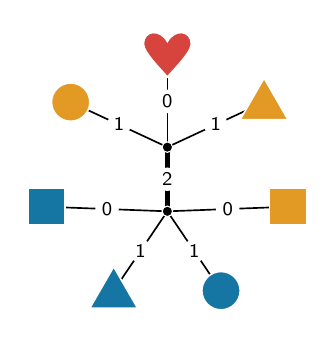
\begin{tikzpicture}[x=1.0cm,y=1.0cm,baseline=(current bounding box.center)]
\coordinate (v1) at (-1.53153,-0.34956);
\coordinate (v2) at (-0.68160,-1.41535);
\coordinate (v3) at (0.68160,-1.41535);
\coordinate (v4) at (1.53153,-0.34956);
\coordinate (v5) at (1.22819,0.97945);
\coordinate (v6) at (-1.22819,0.97945);
\coordinate (v7) at (0.00000,1.57092);
\coordinate (v8) at (-0.00000,0.40755);
\coordinate (v9) at (0.00000,-0.40755);
\draw[g2tree internal] (v8)--(v9);
\draw[g2tree pendant] (v1)--(v9);
\draw[g2tree pendant] (v2)--(v9);
\draw[g2tree pendant] (v3)--(v9);
\draw[g2tree pendant] (v4)--(v9);
\draw[g2tree pendant] (v5)--(v8);
\draw[g2tree pendant] (v6)--(v8);
\draw[g2tree pendant] (v7)--(v8);
\node[g2tree weight,font={\sffamily\fontsize{7.5}{8}\selectfont}] at (0.00000,0.00000) {2};
\node[g2tree weight,font={\sffamily\fontsize{7.5}{8}\selectfont}] at (-0.76577,-0.37856) {0};
\node[g2tree weight,font={\sffamily\fontsize{7.5}{8}\selectfont}] at (-0.34080,-0.91145) {1};
\node[g2tree weight,font={\sffamily\fontsize{7.5}{8}\selectfont}] at (0.34080,-0.91145) {1};
\node[g2tree weight,font={\sffamily\fontsize{7.5}{8}\selectfont}] at (0.76577,-0.37856) {0};
\node[g2tree weight,font={\sffamily\fontsize{7.5}{8}\selectfont}] at (0.61410,0.69350) {1};
\node[g2tree weight,font={\sffamily\fontsize{7.5}{8}\selectfont}] at (-0.61410,0.69350) {1};
\node[g2tree weight,font={\sffamily\fontsize{7.5}{8}\selectfont}] at (0.00000,0.98924) {0};
\node[g2tree vertex] at (v8) {};
\node[g2tree vertex] at (v9) {};
\node[g2tree dark,rectangle,minimum size=4.657500000000001mm,font={\sffamily\fontsize{9}{9}\selectfont\bfseries}] at (v1) {};
\begin{scope}[shift={(v2)},scale=1.0125000000000002,transform shape]
\path[fill=g2TaxonBlue,draw=white,line width=.55pt,line join=round] (0mm,3.0mm)--(-3.0mm,-2.2mm)--(3.0mm,-2.2mm)--cycle;
\end{scope}
\node[g2tree dark,circle,minimum size=4.86mm,font={\sffamily\fontsize{9}{9}\selectfont\bfseries}] at (v3) {};
\node[g2tree light,rectangle,minimum size=4.657500000000001mm,font={\sffamily\fontsize{9}{9}\selectfont\bfseries}] at (v4) {};
\begin{scope}[shift={(v5)},scale=1.0125000000000002,transform shape]
\path[fill=g2TaxonYellow,draw=white,line width=.55pt,line join=round] (0mm,3.0mm)--(-3.0mm,-2.2mm)--(3.0mm,-2.2mm)--cycle;
\end{scope}
\node[g2tree light,circle,minimum size=4.86mm,font={\sffamily\fontsize{9}{9}\selectfont\bfseries}] at (v6) {};
\begin{scope}[shift={(v7)},scale=1.0125000000000002,transform shape]
\path[fill=g2HeartRed,draw=white,line width=.55pt]
  (0mm,-2.7mm)..controls(-.45mm,-2.1mm)and(-3.0mm,.35mm)..(-3.0mm,1.45mm)
  ..controls(-3.0mm,3.2mm)and(-.9mm,3.4mm)..(0mm,1.75mm)
  ..controls(.9mm,3.4mm)and(3.0mm,3.2mm)..(3.0mm,1.45mm)
  ..controls(3.0mm,.35mm)and(.45mm,-2.1mm)..(0mm,-2.7mm)--cycle;
\end{scope}
\end{tikzpicture}
\endgroup
\par}
\end{minipage}
 & 
\begin{minipage}[t][4.1325cm][t]{\linewidth}
\noindent\textcolor{g2TreeRule}{\rule{\linewidth}{1pt}}\par
\noindent\textcolor[HTML]{000000}{\smash[b]{\textpdfrender{TextRenderingMode=FillStroke,LineWidth=.5pt}{\Large\bfseries\boldmath \(\alpha_2\)}{\large(3)}}}\par
\vskip -2.5mm
{\centering
\begingroup
\definecolor{g2TaxonBlue}{HTML}{1676A3}
\definecolor{g2TaxonYellow}{HTML}{E39A24}
\definecolor{g2HeartRed}{HTML}{D7443E}
\tikzset{
  g2tree pendant/.style={draw=black,line width=.6pt,line cap=round},
  g2tree internal/.style={draw=black,line width=2pt,line cap=round},
  g2tree vertex/.style={circle,fill=black,draw=white,line width=.4pt,inner sep=0pt,minimum size=3.8pt},
  g2tree dark/.style={fill=g2TaxonBlue,draw=white,line width=.55pt,text=white,inner sep=0pt},
  g2tree light/.style={fill=g2TaxonYellow,draw=white,line width=.55pt,text=white,inner sep=0pt},
  g2tree weight/.style={circle,fill=white,draw=none,text=black,inner sep=.15pt,minimum size=8.5pt},
  g2tree aligned pendant/.style={fill=white,text=black,inner sep=.7pt,sloped,above=1pt,font={\sffamily\fontsize{7.5}{8}\selectfont}},
  g2tree aligned internal/.style={fill=white,text=black,inner sep=1pt,sloped,above=1pt,font={\sffamily\fontsize{7.5}{8}\selectfont\bfseries}},
}
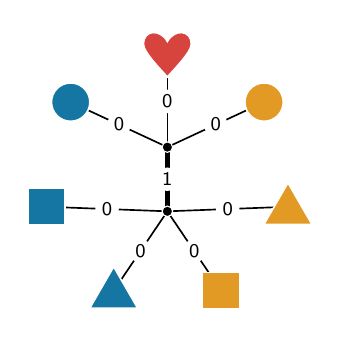
\begin{tikzpicture}[x=1.0cm,y=1.0cm,baseline=(current bounding box.center)]
\coordinate (v1) at (-1.53153,-0.34956);
\coordinate (v2) at (-0.68160,-1.41535);
\coordinate (v3) at (-1.22819,0.97945);
\coordinate (v4) at (0.68160,-1.41535);
\coordinate (v5) at (1.53153,-0.34956);
\coordinate (v6) at (1.22819,0.97945);
\coordinate (v7) at (0.00000,1.57092);
\coordinate (v8) at (-0.00000,0.40755);
\coordinate (v9) at (0.00000,-0.40755);
\draw[g2tree internal] (v8)--(v9);
\draw[g2tree pendant] (v1)--(v9);
\draw[g2tree pendant] (v2)--(v9);
\draw[g2tree pendant] (v3)--(v8);
\draw[g2tree pendant] (v4)--(v9);
\draw[g2tree pendant] (v5)--(v9);
\draw[g2tree pendant] (v6)--(v8);
\draw[g2tree pendant] (v7)--(v8);
\node[g2tree weight,font={\sffamily\fontsize{7.5}{8}\selectfont}] at (0.00000,0.00000) {1};
\node[g2tree weight,font={\sffamily\fontsize{7.5}{8}\selectfont}] at (-0.76577,-0.37856) {0};
\node[g2tree weight,font={\sffamily\fontsize{7.5}{8}\selectfont}] at (-0.34080,-0.91145) {0};
\node[g2tree weight,font={\sffamily\fontsize{7.5}{8}\selectfont}] at (-0.61410,0.69350) {0};
\node[g2tree weight,font={\sffamily\fontsize{7.5}{8}\selectfont}] at (0.34080,-0.91145) {0};
\node[g2tree weight,font={\sffamily\fontsize{7.5}{8}\selectfont}] at (0.76577,-0.37856) {0};
\node[g2tree weight,font={\sffamily\fontsize{7.5}{8}\selectfont}] at (0.61410,0.69350) {0};
\node[g2tree weight,font={\sffamily\fontsize{7.5}{8}\selectfont}] at (0.00000,0.98924) {0};
\node[g2tree vertex] at (v8) {};
\node[g2tree vertex] at (v9) {};
\node[g2tree dark,rectangle,minimum size=4.657500000000001mm,font={\sffamily\fontsize{9}{9}\selectfont\bfseries}] at (v1) {};
\begin{scope}[shift={(v2)},scale=1.0125000000000002,transform shape]
\path[fill=g2TaxonBlue,draw=white,line width=.55pt,line join=round] (0mm,3.0mm)--(-3.0mm,-2.2mm)--(3.0mm,-2.2mm)--cycle;
\end{scope}
\node[g2tree dark,circle,minimum size=4.86mm,font={\sffamily\fontsize{9}{9}\selectfont\bfseries}] at (v3) {};
\node[g2tree light,rectangle,minimum size=4.657500000000001mm,font={\sffamily\fontsize{9}{9}\selectfont\bfseries}] at (v4) {};
\begin{scope}[shift={(v5)},scale=1.0125000000000002,transform shape]
\path[fill=g2TaxonYellow,draw=white,line width=.55pt,line join=round] (0mm,3.0mm)--(-3.0mm,-2.2mm)--(3.0mm,-2.2mm)--cycle;
\end{scope}
\node[g2tree light,circle,minimum size=4.86mm,font={\sffamily\fontsize{9}{9}\selectfont\bfseries}] at (v6) {};
\begin{scope}[shift={(v7)},scale=1.0125000000000002,transform shape]
\path[fill=g2HeartRed,draw=white,line width=.55pt]
  (0mm,-2.7mm)..controls(-.45mm,-2.1mm)and(-3.0mm,.35mm)..(-3.0mm,1.45mm)
  ..controls(-3.0mm,3.2mm)and(-.9mm,3.4mm)..(0mm,1.75mm)
  ..controls(.9mm,3.4mm)and(3.0mm,3.2mm)..(3.0mm,1.45mm)
  ..controls(3.0mm,.35mm)and(.45mm,-2.1mm)..(0mm,-2.7mm)--cycle;
\end{scope}
\end{tikzpicture}
\endgroup
\par}
\end{minipage}
 & 
\begin{minipage}[t][4.1325cm][t]{\linewidth}
\noindent\textcolor{g2TreeRule}{\rule{\linewidth}{1pt}}\par
\noindent\textcolor[HTML]{000000}{\smash[b]{\textpdfrender{TextRenderingMode=FillStroke,LineWidth=.5pt}{\Large\bfseries\boldmath \(\alpha_3\)}{\large(6)}}}\par
\vskip -2.5mm
{\centering
\begingroup
\definecolor{g2TaxonBlue}{HTML}{1676A3}
\definecolor{g2TaxonYellow}{HTML}{E39A24}
\definecolor{g2HeartRed}{HTML}{D7443E}
\tikzset{
  g2tree pendant/.style={draw=black,line width=.6pt,line cap=round},
  g2tree internal/.style={draw=black,line width=2pt,line cap=round},
  g2tree vertex/.style={circle,fill=black,draw=white,line width=.4pt,inner sep=0pt,minimum size=3.8pt},
  g2tree dark/.style={fill=g2TaxonBlue,draw=white,line width=.55pt,text=white,inner sep=0pt},
  g2tree light/.style={fill=g2TaxonYellow,draw=white,line width=.55pt,text=white,inner sep=0pt},
  g2tree weight/.style={circle,fill=white,draw=none,text=black,inner sep=.15pt,minimum size=8.5pt},
  g2tree aligned pendant/.style={fill=white,text=black,inner sep=.7pt,sloped,above=1pt,font={\sffamily\fontsize{7.5}{8}\selectfont}},
  g2tree aligned internal/.style={fill=white,text=black,inner sep=1pt,sloped,above=1pt,font={\sffamily\fontsize{7.5}{8}\selectfont\bfseries}},
}
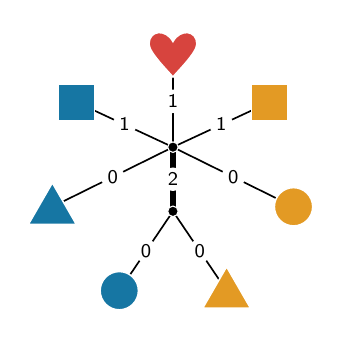
\begin{tikzpicture}[x=1.0cm,y=1.0cm,baseline=(current bounding box.center)]
\coordinate (v1) at (-1.22819,0.97945);
\coordinate (v2) at (-1.53153,-0.34956);
\coordinate (v3) at (-0.68160,-1.41535);
\coordinate (v4) at (1.22819,0.97945);
\coordinate (v5) at (0.68160,-1.41535);
\coordinate (v6) at (1.53153,-0.34956);
\coordinate (v7) at (0.00000,1.57092);
\coordinate (v8) at (0.00000,-0.40755);
\coordinate (v9) at (-0.00000,0.40755);
\draw[g2tree internal] (v8)--(v9);
\draw[g2tree pendant] (v1)--(v9);
\draw[g2tree pendant] (v2)--(v9);
\draw[g2tree pendant] (v3)--(v8);
\draw[g2tree pendant] (v4)--(v9);
\draw[g2tree pendant] (v5)--(v8);
\draw[g2tree pendant] (v6)--(v9);
\draw[g2tree pendant] (v7)--(v9);
\node[g2tree weight,font={\sffamily\fontsize{7.5}{8}\selectfont}] at (0.00000,0.00000) {2};
\node[g2tree weight,font={\sffamily\fontsize{7.5}{8}\selectfont}] at (-0.61410,0.69350) {1};
\node[g2tree weight,font={\sffamily\fontsize{7.5}{8}\selectfont}] at (-0.76577,0.02899) {0};
\node[g2tree weight,font={\sffamily\fontsize{7.5}{8}\selectfont}] at (-0.34080,-0.91145) {0};
\node[g2tree weight,font={\sffamily\fontsize{7.5}{8}\selectfont}] at (0.61410,0.69350) {1};
\node[g2tree weight,font={\sffamily\fontsize{7.5}{8}\selectfont}] at (0.34080,-0.91145) {0};
\node[g2tree weight,font={\sffamily\fontsize{7.5}{8}\selectfont}] at (0.76577,0.02899) {0};
\node[g2tree weight,font={\sffamily\fontsize{7.5}{8}\selectfont}] at (0.00000,0.98924) {1};
\node[g2tree vertex] at (v8) {};
\node[g2tree vertex] at (v9) {};
\node[g2tree dark,rectangle,minimum size=4.657500000000001mm,font={\sffamily\fontsize{9}{9}\selectfont\bfseries}] at (v1) {};
\begin{scope}[shift={(v2)},scale=1.0125000000000002,transform shape]
\path[fill=g2TaxonBlue,draw=white,line width=.55pt,line join=round] (0mm,3.0mm)--(-3.0mm,-2.2mm)--(3.0mm,-2.2mm)--cycle;
\end{scope}
\node[g2tree dark,circle,minimum size=4.86mm,font={\sffamily\fontsize{9}{9}\selectfont\bfseries}] at (v3) {};
\node[g2tree light,rectangle,minimum size=4.657500000000001mm,font={\sffamily\fontsize{9}{9}\selectfont\bfseries}] at (v4) {};
\begin{scope}[shift={(v5)},scale=1.0125000000000002,transform shape]
\path[fill=g2TaxonYellow,draw=white,line width=.55pt,line join=round] (0mm,3.0mm)--(-3.0mm,-2.2mm)--(3.0mm,-2.2mm)--cycle;
\end{scope}
\node[g2tree light,circle,minimum size=4.86mm,font={\sffamily\fontsize{9}{9}\selectfont\bfseries}] at (v6) {};
\begin{scope}[shift={(v7)},scale=1.0125000000000002,transform shape]
\path[fill=g2HeartRed,draw=white,line width=.55pt]
  (0mm,-2.7mm)..controls(-.45mm,-2.1mm)and(-3.0mm,.35mm)..(-3.0mm,1.45mm)
  ..controls(-3.0mm,3.2mm)and(-.9mm,3.4mm)..(0mm,1.75mm)
  ..controls(.9mm,3.4mm)and(3.0mm,3.2mm)..(3.0mm,1.45mm)
  ..controls(3.0mm,.35mm)and(.45mm,-2.1mm)..(0mm,-2.7mm)--cycle;
\end{scope}
\end{tikzpicture}
\endgroup
\par}
\end{minipage}
\\[0.19mm]
\begin{minipage}[t][4.1325cm][t]{\linewidth}
\noindent\textcolor{g2TreeRule}{\rule{\linewidth}{1pt}}\par
\noindent\textcolor[HTML]{000000}{\smash[b]{\textpdfrender{TextRenderingMode=FillStroke,LineWidth=.5pt}{\Large\bfseries\boldmath \(\alpha_4\)}{\large(3)}}}\par
\vskip -2.5mm
{\centering
\begingroup
\definecolor{g2TaxonBlue}{HTML}{1676A3}
\definecolor{g2TaxonYellow}{HTML}{E39A24}
\definecolor{g2HeartRed}{HTML}{D7443E}
\tikzset{
  g2tree pendant/.style={draw=black,line width=.6pt,line cap=round},
  g2tree internal/.style={draw=black,line width=2pt,line cap=round},
  g2tree vertex/.style={circle,fill=black,draw=white,line width=.4pt,inner sep=0pt,minimum size=3.8pt},
  g2tree dark/.style={fill=g2TaxonBlue,draw=white,line width=.55pt,text=white,inner sep=0pt},
  g2tree light/.style={fill=g2TaxonYellow,draw=white,line width=.55pt,text=white,inner sep=0pt},
  g2tree weight/.style={circle,fill=white,draw=none,text=black,inner sep=.15pt,minimum size=8.5pt},
  g2tree aligned pendant/.style={fill=white,text=black,inner sep=.7pt,sloped,above=1pt,font={\sffamily\fontsize{7.5}{8}\selectfont}},
  g2tree aligned internal/.style={fill=white,text=black,inner sep=1pt,sloped,above=1pt,font={\sffamily\fontsize{7.5}{8}\selectfont\bfseries}},
}
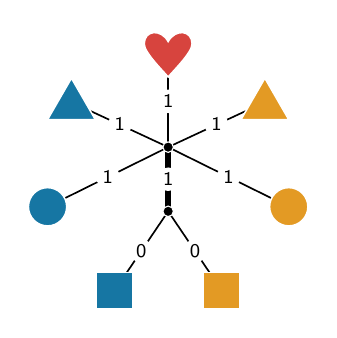
\begin{tikzpicture}[x=1.0cm,y=1.0cm,baseline=(current bounding box.center)]
\coordinate (v1) at (-0.68160,-1.41535);
\coordinate (v2) at (-1.22819,0.97945);
\coordinate (v3) at (-1.53153,-0.34956);
\coordinate (v4) at (0.68160,-1.41535);
\coordinate (v5) at (1.22819,0.97945);
\coordinate (v6) at (1.53153,-0.34956);
\coordinate (v7) at (0.00000,1.57092);
\coordinate (v8) at (0.00000,-0.40755);
\coordinate (v9) at (-0.00000,0.40755);
\draw[g2tree internal] (v8)--(v9);
\draw[g2tree pendant] (v1)--(v8);
\draw[g2tree pendant] (v2)--(v9);
\draw[g2tree pendant] (v3)--(v9);
\draw[g2tree pendant] (v4)--(v8);
\draw[g2tree pendant] (v5)--(v9);
\draw[g2tree pendant] (v6)--(v9);
\draw[g2tree pendant] (v7)--(v9);
\node[g2tree weight,font={\sffamily\fontsize{7.5}{8}\selectfont}] at (0.00000,0.00000) {1};
\node[g2tree weight,font={\sffamily\fontsize{7.5}{8}\selectfont}] at (-0.34080,-0.91145) {0};
\node[g2tree weight,font={\sffamily\fontsize{7.5}{8}\selectfont}] at (-0.61410,0.69350) {1};
\node[g2tree weight,font={\sffamily\fontsize{7.5}{8}\selectfont}] at (-0.76577,0.02899) {1};
\node[g2tree weight,font={\sffamily\fontsize{7.5}{8}\selectfont}] at (0.34080,-0.91145) {0};
\node[g2tree weight,font={\sffamily\fontsize{7.5}{8}\selectfont}] at (0.61410,0.69350) {1};
\node[g2tree weight,font={\sffamily\fontsize{7.5}{8}\selectfont}] at (0.76577,0.02899) {1};
\node[g2tree weight,font={\sffamily\fontsize{7.5}{8}\selectfont}] at (0.00000,0.98924) {1};
\node[g2tree vertex] at (v8) {};
\node[g2tree vertex] at (v9) {};
\node[g2tree dark,rectangle,minimum size=4.657500000000001mm,font={\sffamily\fontsize{9}{9}\selectfont\bfseries}] at (v1) {};
\begin{scope}[shift={(v2)},scale=1.0125000000000002,transform shape]
\path[fill=g2TaxonBlue,draw=white,line width=.55pt,line join=round] (0mm,3.0mm)--(-3.0mm,-2.2mm)--(3.0mm,-2.2mm)--cycle;
\end{scope}
\node[g2tree dark,circle,minimum size=4.86mm,font={\sffamily\fontsize{9}{9}\selectfont\bfseries}] at (v3) {};
\node[g2tree light,rectangle,minimum size=4.657500000000001mm,font={\sffamily\fontsize{9}{9}\selectfont\bfseries}] at (v4) {};
\begin{scope}[shift={(v5)},scale=1.0125000000000002,transform shape]
\path[fill=g2TaxonYellow,draw=white,line width=.55pt,line join=round] (0mm,3.0mm)--(-3.0mm,-2.2mm)--(3.0mm,-2.2mm)--cycle;
\end{scope}
\node[g2tree light,circle,minimum size=4.86mm,font={\sffamily\fontsize{9}{9}\selectfont\bfseries}] at (v6) {};
\begin{scope}[shift={(v7)},scale=1.0125000000000002,transform shape]
\path[fill=g2HeartRed,draw=white,line width=.55pt]
  (0mm,-2.7mm)..controls(-.45mm,-2.1mm)and(-3.0mm,.35mm)..(-3.0mm,1.45mm)
  ..controls(-3.0mm,3.2mm)and(-.9mm,3.4mm)..(0mm,1.75mm)
  ..controls(.9mm,3.4mm)and(3.0mm,3.2mm)..(3.0mm,1.45mm)
  ..controls(3.0mm,.35mm)and(.45mm,-2.1mm)..(0mm,-2.7mm)--cycle;
\end{scope}
\end{tikzpicture}
\endgroup
\par}
\end{minipage}
 & 
\begin{minipage}[t][4.1325cm][t]{\linewidth}
\noindent\textcolor{g2TreeRule}{\rule{\linewidth}{1pt}}\par
\noindent\textcolor[HTML]{000000}{\smash[b]{\textpdfrender{TextRenderingMode=FillStroke,LineWidth=.5pt}{\Large\bfseries\boldmath \(\alpha_5\)}{\large(2)}}}\par
\vskip -2.5mm
{\centering
\begingroup
\definecolor{g2TaxonBlue}{HTML}{1676A3}
\definecolor{g2TaxonYellow}{HTML}{E39A24}
\definecolor{g2HeartRed}{HTML}{D7443E}
\tikzset{
  g2tree pendant/.style={draw=black,line width=.6pt,line cap=round},
  g2tree internal/.style={draw=black,line width=2pt,line cap=round},
  g2tree vertex/.style={circle,fill=black,draw=white,line width=.4pt,inner sep=0pt,minimum size=3.8pt},
  g2tree dark/.style={fill=g2TaxonBlue,draw=white,line width=.55pt,text=white,inner sep=0pt},
  g2tree light/.style={fill=g2TaxonYellow,draw=white,line width=.55pt,text=white,inner sep=0pt},
  g2tree weight/.style={circle,fill=white,draw=none,text=black,inner sep=.15pt,minimum size=8.5pt},
  g2tree aligned pendant/.style={fill=white,text=black,inner sep=.7pt,sloped,above=1pt,font={\sffamily\fontsize{7.5}{8}\selectfont}},
  g2tree aligned internal/.style={fill=white,text=black,inner sep=1pt,sloped,above=1pt,font={\sffamily\fontsize{7.5}{8}\selectfont\bfseries}},
}
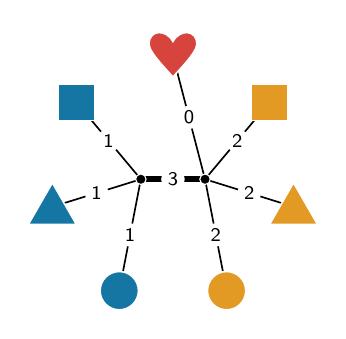
\begin{tikzpicture}[x=1.0cm,y=1.0cm,baseline=(current bounding box.center)]
\coordinate (v1) at (-1.22819,0.97945);
\coordinate (v2) at (-1.53153,-0.34956);
\coordinate (v3) at (-0.68160,-1.41535);
\coordinate (v4) at (1.22819,0.97945);
\coordinate (v5) at (1.53153,-0.34956);
\coordinate (v6) at (0.68160,-1.41535);
\coordinate (v7) at (0.00000,1.57092);
\coordinate (v8) at (-0.40755,0.00000);
\coordinate (v9) at (0.40755,0.00000);
\draw[g2tree internal] (v8)--(v9);
\draw[g2tree pendant] (v1)--(v8);
\draw[g2tree pendant] (v2)--(v8);
\draw[g2tree pendant] (v3)--(v8);
\draw[g2tree pendant] (v4)--(v9);
\draw[g2tree pendant] (v5)--(v9);
\draw[g2tree pendant] (v6)--(v9);
\draw[g2tree pendant] (v7)--(v9);
\node[g2tree weight,font={\sffamily\fontsize{7.5}{8}\selectfont}] at (0.00000,0.00000) {3};
\node[g2tree weight,font={\sffamily\fontsize{7.5}{8}\selectfont}] at (-0.81787,0.48973) {1};
\node[g2tree weight,font={\sffamily\fontsize{7.5}{8}\selectfont}] at (-0.96954,-0.17478) {1};
\node[g2tree weight,font={\sffamily\fontsize{7.5}{8}\selectfont}] at (-0.54457,-0.70768) {1};
\node[g2tree weight,font={\sffamily\fontsize{7.5}{8}\selectfont}] at (0.81787,0.48973) {2};
\node[g2tree weight,font={\sffamily\fontsize{7.5}{8}\selectfont}] at (0.96954,-0.17478) {2};
\node[g2tree weight,font={\sffamily\fontsize{7.5}{8}\selectfont}] at (0.54457,-0.70768) {2};
\node[g2tree weight,font={\sffamily\fontsize{7.5}{8}\selectfont}] at (0.20378,0.78546) {0};
\node[g2tree vertex] at (v8) {};
\node[g2tree vertex] at (v9) {};
\node[g2tree dark,rectangle,minimum size=4.657500000000001mm,font={\sffamily\fontsize{9}{9}\selectfont\bfseries}] at (v1) {};
\begin{scope}[shift={(v2)},scale=1.0125000000000002,transform shape]
\path[fill=g2TaxonBlue,draw=white,line width=.55pt,line join=round] (0mm,3.0mm)--(-3.0mm,-2.2mm)--(3.0mm,-2.2mm)--cycle;
\end{scope}
\node[g2tree dark,circle,minimum size=4.86mm,font={\sffamily\fontsize{9}{9}\selectfont\bfseries}] at (v3) {};
\node[g2tree light,rectangle,minimum size=4.657500000000001mm,font={\sffamily\fontsize{9}{9}\selectfont\bfseries}] at (v4) {};
\begin{scope}[shift={(v5)},scale=1.0125000000000002,transform shape]
\path[fill=g2TaxonYellow,draw=white,line width=.55pt,line join=round] (0mm,3.0mm)--(-3.0mm,-2.2mm)--(3.0mm,-2.2mm)--cycle;
\end{scope}
\node[g2tree light,circle,minimum size=4.86mm,font={\sffamily\fontsize{9}{9}\selectfont\bfseries}] at (v6) {};
\begin{scope}[shift={(v7)},scale=1.0125000000000002,transform shape]
\path[fill=g2HeartRed,draw=white,line width=.55pt]
  (0mm,-2.7mm)..controls(-.45mm,-2.1mm)and(-3.0mm,.35mm)..(-3.0mm,1.45mm)
  ..controls(-3.0mm,3.2mm)and(-.9mm,3.4mm)..(0mm,1.75mm)
  ..controls(.9mm,3.4mm)and(3.0mm,3.2mm)..(3.0mm,1.45mm)
  ..controls(3.0mm,.35mm)and(.45mm,-2.1mm)..(0mm,-2.7mm)--cycle;
\end{scope}
\end{tikzpicture}
\endgroup
\par}
\end{minipage}
 & 
\begin{minipage}[t][4.1325cm][t]{\linewidth}
\noindent\textcolor{g2TreeRule}{\rule{\linewidth}{1pt}}\par
\noindent\textcolor[HTML]{000000}{\smash[b]{\textpdfrender{TextRenderingMode=FillStroke,LineWidth=.5pt}{\Large\bfseries\boldmath \(\beta_1\)}{\large(12)}}}\par
\vskip -2.5mm
{\centering
\begingroup
\definecolor{g2TaxonBlue}{HTML}{1676A3}
\definecolor{g2TaxonYellow}{HTML}{E39A24}
\definecolor{g2HeartRed}{HTML}{D7443E}
\tikzset{
  g2tree pendant/.style={draw=black,line width=.6pt,line cap=round},
  g2tree internal/.style={draw=black,line width=2pt,line cap=round},
  g2tree vertex/.style={circle,fill=black,draw=white,line width=.4pt,inner sep=0pt,minimum size=3.8pt},
  g2tree dark/.style={fill=g2TaxonBlue,draw=white,line width=.55pt,text=white,inner sep=0pt},
  g2tree light/.style={fill=g2TaxonYellow,draw=white,line width=.55pt,text=white,inner sep=0pt},
  g2tree weight/.style={circle,fill=white,draw=none,text=black,inner sep=.15pt,minimum size=8.5pt},
  g2tree aligned pendant/.style={fill=white,text=black,inner sep=.7pt,sloped,above=1pt,font={\sffamily\fontsize{7.5}{8}\selectfont}},
  g2tree aligned internal/.style={fill=white,text=black,inner sep=1pt,sloped,above=1pt,font={\sffamily\fontsize{7.5}{8}\selectfont\bfseries}},
}
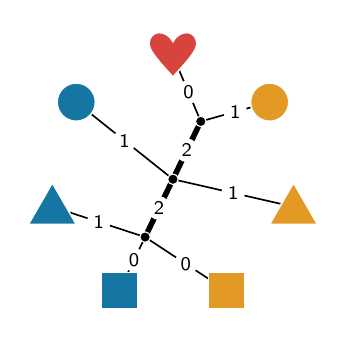
\begin{tikzpicture}[x=1.0cm,y=1.0cm,baseline=(current bounding box.center)]
\coordinate (v1) at (-0.68160,-1.41535);
\coordinate (v2) at (-1.53153,-0.34956);
\coordinate (v3) at (-1.22819,0.97945);
\coordinate (v4) at (0.68160,-1.41535);
\coordinate (v5) at (1.53153,-0.34956);
\coordinate (v6) at (1.22819,0.97945);
\coordinate (v7) at (0.00000,1.57092);
\coordinate (v8) at (0.35366,0.73438);
\coordinate (v9) at (-0.35366,-0.73438);
\coordinate (v10) at (0.00000,0.00000);
\draw[g2tree internal] (v8)--(v10);
\draw[g2tree internal] (v9)--(v10);
\draw[g2tree pendant] (v1)--(v9);
\draw[g2tree pendant] (v2)--(v9);
\draw[g2tree pendant] (v3)--(v10);
\draw[g2tree pendant] (v4)--(v9);
\draw[g2tree pendant] (v5)--(v10);
\draw[g2tree pendant] (v6)--(v8);
\draw[g2tree pendant] (v7)--(v8);
\node[g2tree weight,font={\sffamily\fontsize{7.5}{8}\selectfont}] at (0.17683,0.36719) {2};
\node[g2tree weight,font={\sffamily\fontsize{7.5}{8}\selectfont}] at (-0.17683,-0.36719) {2};
\node[g2tree weight,font={\sffamily\fontsize{7.5}{8}\selectfont}] at (-0.49303,-1.02379) {0};
\node[g2tree weight,font={\sffamily\fontsize{7.5}{8}\selectfont}] at (-0.94260,-0.54197) {1};
\node[g2tree weight,font={\sffamily\fontsize{7.5}{8}\selectfont}] at (-0.61410,0.48973) {1};
\node[g2tree weight,font={\sffamily\fontsize{7.5}{8}\selectfont}] at (0.16397,-1.07486) {0};
\node[g2tree weight,font={\sffamily\fontsize{7.5}{8}\selectfont}] at (0.76577,-0.17478) {1};
\node[g2tree weight,font={\sffamily\fontsize{7.5}{8}\selectfont}] at (0.79093,0.85692) {1};
\node[g2tree weight,font={\sffamily\fontsize{7.5}{8}\selectfont}] at (0.19632,1.10655) {0};
\node[g2tree vertex] at (v8) {};
\node[g2tree vertex] at (v9) {};
\node[g2tree vertex] at (v10) {};
\node[g2tree dark,rectangle,minimum size=4.657500000000001mm,font={\sffamily\fontsize{9}{9}\selectfont\bfseries}] at (v1) {};
\begin{scope}[shift={(v2)},scale=1.0125000000000002,transform shape]
\path[fill=g2TaxonBlue,draw=white,line width=.55pt,line join=round] (0mm,3.0mm)--(-3.0mm,-2.2mm)--(3.0mm,-2.2mm)--cycle;
\end{scope}
\node[g2tree dark,circle,minimum size=4.86mm,font={\sffamily\fontsize{9}{9}\selectfont\bfseries}] at (v3) {};
\node[g2tree light,rectangle,minimum size=4.657500000000001mm,font={\sffamily\fontsize{9}{9}\selectfont\bfseries}] at (v4) {};
\begin{scope}[shift={(v5)},scale=1.0125000000000002,transform shape]
\path[fill=g2TaxonYellow,draw=white,line width=.55pt,line join=round] (0mm,3.0mm)--(-3.0mm,-2.2mm)--(3.0mm,-2.2mm)--cycle;
\end{scope}
\node[g2tree light,circle,minimum size=4.86mm,font={\sffamily\fontsize{9}{9}\selectfont\bfseries}] at (v6) {};
\begin{scope}[shift={(v7)},scale=1.0125000000000002,transform shape]
\path[fill=g2HeartRed,draw=white,line width=.55pt]
  (0mm,-2.7mm)..controls(-.45mm,-2.1mm)and(-3.0mm,.35mm)..(-3.0mm,1.45mm)
  ..controls(-3.0mm,3.2mm)and(-.9mm,3.4mm)..(0mm,1.75mm)
  ..controls(.9mm,3.4mm)and(3.0mm,3.2mm)..(3.0mm,1.45mm)
  ..controls(3.0mm,.35mm)and(.45mm,-2.1mm)..(0mm,-2.7mm)--cycle;
\end{scope}
\end{tikzpicture}
\endgroup
\par}
\end{minipage}
\\[0.19mm]
\begin{minipage}[t][4.1325cm][t]{\linewidth}
\noindent\textcolor{g2TreeRule}{\rule{\linewidth}{1pt}}\par
\noindent\textcolor[HTML]{000000}{\smash[b]{\textpdfrender{TextRenderingMode=FillStroke,LineWidth=.5pt}{\Large\bfseries\boldmath \(\beta_2\)}{\large(6)}}}\par
\vskip -2.5mm
{\centering
\begingroup
\definecolor{g2TaxonBlue}{HTML}{1676A3}
\definecolor{g2TaxonYellow}{HTML}{E39A24}
\definecolor{g2HeartRed}{HTML}{D7443E}
\tikzset{
  g2tree pendant/.style={draw=black,line width=.6pt,line cap=round},
  g2tree internal/.style={draw=black,line width=2pt,line cap=round},
  g2tree vertex/.style={circle,fill=black,draw=white,line width=.4pt,inner sep=0pt,minimum size=3.8pt},
  g2tree dark/.style={fill=g2TaxonBlue,draw=white,line width=.55pt,text=white,inner sep=0pt},
  g2tree light/.style={fill=g2TaxonYellow,draw=white,line width=.55pt,text=white,inner sep=0pt},
  g2tree weight/.style={circle,fill=white,draw=none,text=black,inner sep=.15pt,minimum size=8.5pt},
  g2tree aligned pendant/.style={fill=white,text=black,inner sep=.7pt,sloped,above=1pt,font={\sffamily\fontsize{7.5}{8}\selectfont}},
  g2tree aligned internal/.style={fill=white,text=black,inner sep=1pt,sloped,above=1pt,font={\sffamily\fontsize{7.5}{8}\selectfont\bfseries}},
}
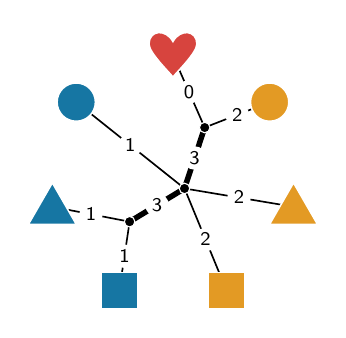
\begin{tikzpicture}[x=1.0cm,y=1.0cm,baseline=(current bounding box.center)]
\coordinate (v1) at (-0.68160,-1.41535);
\coordinate (v2) at (-1.53153,-0.34956);
\coordinate (v3) at (-1.22819,0.97945);
\coordinate (v4) at (0.68160,-1.41535);
\coordinate (v5) at (1.53153,-0.34956);
\coordinate (v6) at (1.22819,0.97945);
\coordinate (v7) at (0.00000,1.57092);
\coordinate (v8) at (-0.55031,-0.53932);
\coordinate (v9) at (0.40334,0.65653);
\coordinate (v10) at (0.14697,-0.11720);
\draw[g2tree internal] (v8)--(v10);
\draw[g2tree internal] (v9)--(v10);
\draw[g2tree pendant] (v1)--(v8);
\draw[g2tree pendant] (v2)--(v8);
\draw[g2tree pendant] (v3)--(v10);
\draw[g2tree pendant] (v4)--(v10);
\draw[g2tree pendant] (v5)--(v10);
\draw[g2tree pendant] (v6)--(v9);
\draw[g2tree pendant] (v7)--(v9);
\node[g2tree weight,font={\sffamily\fontsize{7.5}{8}\selectfont}] at (-0.20167,-0.32826) {3};
\node[g2tree weight,font={\sffamily\fontsize{7.5}{8}\selectfont}] at (0.27516,0.26966) {3};
\node[g2tree weight,font={\sffamily\fontsize{7.5}{8}\selectfont}] at (-0.61596,-0.97734) {1};
\node[g2tree weight,font={\sffamily\fontsize{7.5}{8}\selectfont}] at (-1.04092,-0.44444) {1};
\node[g2tree weight,font={\sffamily\fontsize{7.5}{8}\selectfont}] at (-0.54061,0.43112) {1};
\node[g2tree weight,font={\sffamily\fontsize{7.5}{8}\selectfont}] at (0.41428,-0.76628) {2};
\node[g2tree weight,font={\sffamily\fontsize{7.5}{8}\selectfont}] at (0.83925,-0.23338) {2};
\node[g2tree weight,font={\sffamily\fontsize{7.5}{8}\selectfont}] at (0.81577,0.81799) {2};
\node[g2tree weight,font={\sffamily\fontsize{7.5}{8}\selectfont}] at (0.20347,1.10964) {0};
\node[g2tree vertex] at (v8) {};
\node[g2tree vertex] at (v9) {};
\node[g2tree vertex] at (v10) {};
\node[g2tree dark,rectangle,minimum size=4.657500000000001mm,font={\sffamily\fontsize{9}{9}\selectfont\bfseries}] at (v1) {};
\begin{scope}[shift={(v2)},scale=1.0125000000000002,transform shape]
\path[fill=g2TaxonBlue,draw=white,line width=.55pt,line join=round] (0mm,3.0mm)--(-3.0mm,-2.2mm)--(3.0mm,-2.2mm)--cycle;
\end{scope}
\node[g2tree dark,circle,minimum size=4.86mm,font={\sffamily\fontsize{9}{9}\selectfont\bfseries}] at (v3) {};
\node[g2tree light,rectangle,minimum size=4.657500000000001mm,font={\sffamily\fontsize{9}{9}\selectfont\bfseries}] at (v4) {};
\begin{scope}[shift={(v5)},scale=1.0125000000000002,transform shape]
\path[fill=g2TaxonYellow,draw=white,line width=.55pt,line join=round] (0mm,3.0mm)--(-3.0mm,-2.2mm)--(3.0mm,-2.2mm)--cycle;
\end{scope}
\node[g2tree light,circle,minimum size=4.86mm,font={\sffamily\fontsize{9}{9}\selectfont\bfseries}] at (v6) {};
\begin{scope}[shift={(v7)},scale=1.0125000000000002,transform shape]
\path[fill=g2HeartRed,draw=white,line width=.55pt]
  (0mm,-2.7mm)..controls(-.45mm,-2.1mm)and(-3.0mm,.35mm)..(-3.0mm,1.45mm)
  ..controls(-3.0mm,3.2mm)and(-.9mm,3.4mm)..(0mm,1.75mm)
  ..controls(.9mm,3.4mm)and(3.0mm,3.2mm)..(3.0mm,1.45mm)
  ..controls(3.0mm,.35mm)and(.45mm,-2.1mm)..(0mm,-2.7mm)--cycle;
\end{scope}
\end{tikzpicture}
\endgroup
\par}
\end{minipage}
 & 
\begin{minipage}[t][4.1325cm][t]{\linewidth}
\noindent\textcolor{g2TreeRule}{\rule{\linewidth}{1pt}}\par
\noindent\textcolor[HTML]{000000}{\smash[b]{\textpdfrender{TextRenderingMode=FillStroke,LineWidth=.5pt}{\Large\bfseries\boldmath \(\gamma_1\)}{\large(6)}}}\par
\vskip -2.5mm
{\centering
\begingroup
\definecolor{g2TaxonBlue}{HTML}{1676A3}
\definecolor{g2TaxonYellow}{HTML}{E39A24}
\definecolor{g2HeartRed}{HTML}{D7443E}
\tikzset{
  g2tree pendant/.style={draw=black,line width=.6pt,line cap=round},
  g2tree internal/.style={draw=black,line width=2pt,line cap=round},
  g2tree vertex/.style={circle,fill=black,draw=white,line width=.4pt,inner sep=0pt,minimum size=3.8pt},
  g2tree dark/.style={fill=g2TaxonBlue,draw=white,line width=.55pt,text=white,inner sep=0pt},
  g2tree light/.style={fill=g2TaxonYellow,draw=white,line width=.55pt,text=white,inner sep=0pt},
  g2tree weight/.style={circle,fill=white,draw=none,text=black,inner sep=.15pt,minimum size=8.5pt},
  g2tree aligned pendant/.style={fill=white,text=black,inner sep=.7pt,sloped,above=1pt,font={\sffamily\fontsize{7.5}{8}\selectfont}},
  g2tree aligned internal/.style={fill=white,text=black,inner sep=1pt,sloped,above=1pt,font={\sffamily\fontsize{7.5}{8}\selectfont\bfseries}},
}
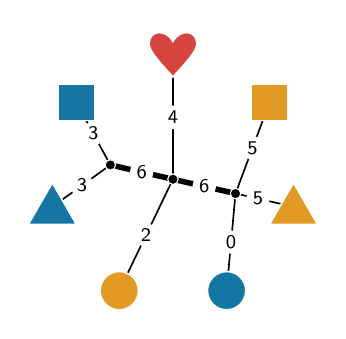
\begin{tikzpicture}[x=1.0cm,y=1.0cm,baseline=(current bounding box.center)]
\coordinate (v1) at (-1.22819,0.97945);
\coordinate (v2) at (-1.53153,-0.34956);
\coordinate (v3) at (0.68160,-1.41535);
\coordinate (v4) at (1.22819,0.97945);
\coordinate (v5) at (1.53153,-0.34956);
\coordinate (v6) at (-0.68160,-1.41535);
\coordinate (v7) at (0.00000,1.57092);
\coordinate (v8) at (-0.79466,0.18138);
\coordinate (v9) at (0.79466,-0.18138);
\coordinate (v10) at (0.00000,0.00000);
\draw[g2tree internal] (v8)--(v10);
\draw[g2tree internal] (v9)--(v10);
\draw[g2tree pendant] (v1)--(v8);
\draw[g2tree pendant] (v2)--(v8);
\draw[g2tree pendant] (v3)--(v9);
\draw[g2tree pendant] (v4)--(v9);
\draw[g2tree pendant] (v5)--(v9);
\draw[g2tree pendant] (v6)--(v10);
\draw[g2tree pendant] (v7)--(v10);
\node[g2tree weight,font={\sffamily\fontsize{7.5}{8}\selectfont}] at (-0.39733,0.09069) {6};
\node[g2tree weight,font={\sffamily\fontsize{7.5}{8}\selectfont}] at (0.39733,-0.09069) {6};
\node[g2tree weight,font={\sffamily\fontsize{7.5}{8}\selectfont}] at (-1.01143,0.58041) {3};
\node[g2tree weight,font={\sffamily\fontsize{7.5}{8}\selectfont}] at (-1.15535,-0.07851) {3};
\node[g2tree weight,font={\sffamily\fontsize{7.5}{8}\selectfont}] at (0.73813,-0.79836) {0};
\node[g2tree weight,font={\sffamily\fontsize{7.5}{8}\selectfont}] at (1.01143,0.39904) {5};
\node[g2tree weight,font={\sffamily\fontsize{7.5}{8}\selectfont}] at (1.07949,-0.24639) {5};
\node[g2tree weight,font={\sffamily\fontsize{7.5}{8}\selectfont}] at (-0.34080,-0.70768) {2};
\node[g2tree weight,font={\sffamily\fontsize{7.5}{8}\selectfont}] at (0.00000,0.78546) {4};
\node[g2tree vertex] at (v8) {};
\node[g2tree vertex] at (v9) {};
\node[g2tree vertex] at (v10) {};
\node[g2tree dark,rectangle,minimum size=4.657500000000001mm,font={\sffamily\fontsize{9}{9}\selectfont\bfseries}] at (v1) {};
\begin{scope}[shift={(v2)},scale=1.0125000000000002,transform shape]
\path[fill=g2TaxonBlue,draw=white,line width=.55pt,line join=round] (0mm,3.0mm)--(-3.0mm,-2.2mm)--(3.0mm,-2.2mm)--cycle;
\end{scope}
\node[g2tree dark,circle,minimum size=4.86mm,font={\sffamily\fontsize{9}{9}\selectfont\bfseries}] at (v3) {};
\node[g2tree light,rectangle,minimum size=4.657500000000001mm,font={\sffamily\fontsize{9}{9}\selectfont\bfseries}] at (v4) {};
\begin{scope}[shift={(v5)},scale=1.0125000000000002,transform shape]
\path[fill=g2TaxonYellow,draw=white,line width=.55pt,line join=round] (0mm,3.0mm)--(-3.0mm,-2.2mm)--(3.0mm,-2.2mm)--cycle;
\end{scope}
\node[g2tree light,circle,minimum size=4.86mm,font={\sffamily\fontsize{9}{9}\selectfont\bfseries}] at (v6) {};
\begin{scope}[shift={(v7)},scale=1.0125000000000002,transform shape]
\path[fill=g2HeartRed,draw=white,line width=.55pt]
  (0mm,-2.7mm)..controls(-.45mm,-2.1mm)and(-3.0mm,.35mm)..(-3.0mm,1.45mm)
  ..controls(-3.0mm,3.2mm)and(-.9mm,3.4mm)..(0mm,1.75mm)
  ..controls(.9mm,3.4mm)and(3.0mm,3.2mm)..(3.0mm,1.45mm)
  ..controls(3.0mm,.35mm)and(.45mm,-2.1mm)..(0mm,-2.7mm)--cycle;
\end{scope}
\end{tikzpicture}
\endgroup
\par}
\end{minipage}
 & 
\begin{minipage}[t][4.1325cm][t]{\linewidth}
\noindent\textcolor{g2TreeRule}{\rule{\linewidth}{1pt}}\par
\noindent\textcolor[HTML]{000000}{\smash[b]{\textpdfrender{TextRenderingMode=FillStroke,LineWidth=.5pt}{\Large\bfseries\boldmath \(\gamma_2\)}{\large(3)}}}\par
\vskip -2.5mm
{\centering
\begingroup
\definecolor{g2TaxonBlue}{HTML}{1676A3}
\definecolor{g2TaxonYellow}{HTML}{E39A24}
\definecolor{g2HeartRed}{HTML}{D7443E}
\tikzset{
  g2tree pendant/.style={draw=black,line width=.6pt,line cap=round},
  g2tree internal/.style={draw=black,line width=2pt,line cap=round},
  g2tree vertex/.style={circle,fill=black,draw=white,line width=.4pt,inner sep=0pt,minimum size=3.8pt},
  g2tree dark/.style={fill=g2TaxonBlue,draw=white,line width=.55pt,text=white,inner sep=0pt},
  g2tree light/.style={fill=g2TaxonYellow,draw=white,line width=.55pt,text=white,inner sep=0pt},
  g2tree weight/.style={circle,fill=white,draw=none,text=black,inner sep=.15pt,minimum size=8.5pt},
  g2tree aligned pendant/.style={fill=white,text=black,inner sep=.7pt,sloped,above=1pt,font={\sffamily\fontsize{7.5}{8}\selectfont}},
  g2tree aligned internal/.style={fill=white,text=black,inner sep=1pt,sloped,above=1pt,font={\sffamily\fontsize{7.5}{8}\selectfont\bfseries}},
}
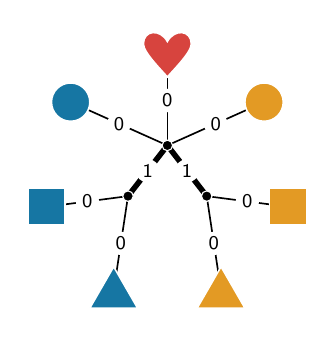
\begin{tikzpicture}[x=1.0cm,y=1.0cm,baseline=(current bounding box.center)]
\coordinate (v1) at (-1.53153,-0.34956);
\coordinate (v2) at (-0.68160,-1.41535);
\coordinate (v3) at (-1.22819,0.97945);
\coordinate (v4) at (1.53153,-0.34956);
\coordinate (v5) at (0.68160,-1.41535);
\coordinate (v6) at (1.22819,0.97945);
\coordinate (v7) at (0.00000,1.57092);
\coordinate (v8) at (-0.49981,-0.21462);
\coordinate (v9) at (0.49981,-0.21462);
\coordinate (v10) at (0.00000,0.42925);
\draw[g2tree internal] (v8)--(v10);
\draw[g2tree internal] (v9)--(v10);
\draw[g2tree pendant] (v1)--(v8);
\draw[g2tree pendant] (v2)--(v8);
\draw[g2tree pendant] (v3)--(v10);
\draw[g2tree pendant] (v4)--(v9);
\draw[g2tree pendant] (v5)--(v9);
\draw[g2tree pendant] (v6)--(v10);
\draw[g2tree pendant] (v7)--(v10);
\node[g2tree weight,font={\sffamily\fontsize{7.5}{8}\selectfont}] at (-0.24991,0.10731) {1};
\node[g2tree weight,font={\sffamily\fontsize{7.5}{8}\selectfont}] at (0.24991,0.10731) {1};
\node[g2tree weight,font={\sffamily\fontsize{7.5}{8}\selectfont}] at (-1.01567,-0.28209) {0};
\node[g2tree weight,font={\sffamily\fontsize{7.5}{8}\selectfont}] at (-0.59071,-0.81499) {0};
\node[g2tree weight,font={\sffamily\fontsize{7.5}{8}\selectfont}] at (-0.61410,0.70435) {0};
\node[g2tree weight,font={\sffamily\fontsize{7.5}{8}\selectfont}] at (1.01567,-0.28209) {0};
\node[g2tree weight,font={\sffamily\fontsize{7.5}{8}\selectfont}] at (0.59071,-0.81499) {0};
\node[g2tree weight,font={\sffamily\fontsize{7.5}{8}\selectfont}] at (0.61410,0.70435) {0};
\node[g2tree weight,font={\sffamily\fontsize{7.5}{8}\selectfont}] at (0.00000,1.00008) {0};
\node[g2tree vertex] at (v8) {};
\node[g2tree vertex] at (v9) {};
\node[g2tree vertex] at (v10) {};
\node[g2tree dark,rectangle,minimum size=4.657500000000001mm,font={\sffamily\fontsize{9}{9}\selectfont\bfseries}] at (v1) {};
\begin{scope}[shift={(v2)},scale=1.0125000000000002,transform shape]
\path[fill=g2TaxonBlue,draw=white,line width=.55pt,line join=round] (0mm,3.0mm)--(-3.0mm,-2.2mm)--(3.0mm,-2.2mm)--cycle;
\end{scope}
\node[g2tree dark,circle,minimum size=4.86mm,font={\sffamily\fontsize{9}{9}\selectfont\bfseries}] at (v3) {};
\node[g2tree light,rectangle,minimum size=4.657500000000001mm,font={\sffamily\fontsize{9}{9}\selectfont\bfseries}] at (v4) {};
\begin{scope}[shift={(v5)},scale=1.0125000000000002,transform shape]
\path[fill=g2TaxonYellow,draw=white,line width=.55pt,line join=round] (0mm,3.0mm)--(-3.0mm,-2.2mm)--(3.0mm,-2.2mm)--cycle;
\end{scope}
\node[g2tree light,circle,minimum size=4.86mm,font={\sffamily\fontsize{9}{9}\selectfont\bfseries}] at (v6) {};
\begin{scope}[shift={(v7)},scale=1.0125000000000002,transform shape]
\path[fill=g2HeartRed,draw=white,line width=.55pt]
  (0mm,-2.7mm)..controls(-.45mm,-2.1mm)and(-3.0mm,.35mm)..(-3.0mm,1.45mm)
  ..controls(-3.0mm,3.2mm)and(-.9mm,3.4mm)..(0mm,1.75mm)
  ..controls(.9mm,3.4mm)and(3.0mm,3.2mm)..(3.0mm,1.45mm)
  ..controls(3.0mm,.35mm)and(.45mm,-2.1mm)..(0mm,-2.7mm)--cycle;
\end{scope}
\end{tikzpicture}
\endgroup
\par}
\end{minipage}
\\[0.19mm]
\begin{minipage}[t][4.1325cm][t]{\linewidth}
\noindent\textcolor{g2TreeRule}{\rule{\linewidth}{1pt}}\par
\noindent\textcolor[HTML]{000000}{\smash[b]{\textpdfrender{TextRenderingMode=FillStroke,LineWidth=.5pt}{\Large\bfseries\boldmath \(\gamma_3\)}{\large(3)}}}\par
\vskip -2.5mm
{\centering
\begingroup
\definecolor{g2TaxonBlue}{HTML}{1676A3}
\definecolor{g2TaxonYellow}{HTML}{E39A24}
\definecolor{g2HeartRed}{HTML}{D7443E}
\tikzset{
  g2tree pendant/.style={draw=black,line width=.6pt,line cap=round},
  g2tree internal/.style={draw=black,line width=2pt,line cap=round},
  g2tree vertex/.style={circle,fill=black,draw=white,line width=.4pt,inner sep=0pt,minimum size=3.8pt},
  g2tree dark/.style={fill=g2TaxonBlue,draw=white,line width=.55pt,text=white,inner sep=0pt},
  g2tree light/.style={fill=g2TaxonYellow,draw=white,line width=.55pt,text=white,inner sep=0pt},
  g2tree weight/.style={circle,fill=white,draw=none,text=black,inner sep=.15pt,minimum size=8.5pt},
  g2tree aligned pendant/.style={fill=white,text=black,inner sep=.7pt,sloped,above=1pt,font={\sffamily\fontsize{7.5}{8}\selectfont}},
  g2tree aligned internal/.style={fill=white,text=black,inner sep=1pt,sloped,above=1pt,font={\sffamily\fontsize{7.5}{8}\selectfont\bfseries}},
}
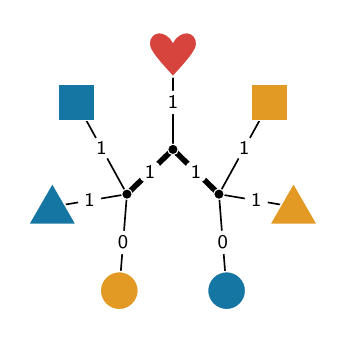
\begin{tikzpicture}[x=1.0cm,y=1.0cm,baseline=(current bounding box.center)]
\coordinate (v1) at (-1.22819,0.97945);
\coordinate (v2) at (-1.53153,-0.34956);
\coordinate (v3) at (0.68160,-1.41535);
\coordinate (v4) at (1.22819,0.97945);
\coordinate (v5) at (1.53153,-0.34956);
\coordinate (v6) at (-0.68160,-1.41535);
\coordinate (v7) at (0.00000,1.57092);
\coordinate (v8) at (-0.58442,-0.18940);
\coordinate (v9) at (0.00000,0.37879);
\coordinate (v10) at (0.58442,-0.18940);
\draw[g2tree internal] (v8)--(v9);
\draw[g2tree internal] (v9)--(v10);
\draw[g2tree pendant] (v1)--(v8);
\draw[g2tree pendant] (v2)--(v8);
\draw[g2tree pendant] (v3)--(v10);
\draw[g2tree pendant] (v4)--(v10);
\draw[g2tree pendant] (v5)--(v10);
\draw[g2tree pendant] (v6)--(v8);
\draw[g2tree pendant] (v7)--(v9);
\node[g2tree weight,font={\sffamily\fontsize{7.5}{8}\selectfont}] at (-0.29221,0.09470) {1};
\node[g2tree weight,font={\sffamily\fontsize{7.5}{8}\selectfont}] at (0.29221,0.09470) {1};
\node[g2tree weight,font={\sffamily\fontsize{7.5}{8}\selectfont}] at (-0.90631,0.39503) {1};
\node[g2tree weight,font={\sffamily\fontsize{7.5}{8}\selectfont}] at (-1.05798,-0.26948) {1};
\node[g2tree weight,font={\sffamily\fontsize{7.5}{8}\selectfont}] at (0.63301,-0.80237) {0};
\node[g2tree weight,font={\sffamily\fontsize{7.5}{8}\selectfont}] at (0.90631,0.39503) {1};
\node[g2tree weight,font={\sffamily\fontsize{7.5}{8}\selectfont}] at (1.05798,-0.26948) {1};
\node[g2tree weight,font={\sffamily\fontsize{7.5}{8}\selectfont}] at (-0.63301,-0.80237) {0};
\node[g2tree weight,font={\sffamily\fontsize{7.5}{8}\selectfont}] at (0.00000,0.97486) {1};
\node[g2tree vertex] at (v8) {};
\node[g2tree vertex] at (v9) {};
\node[g2tree vertex] at (v10) {};
\node[g2tree dark,rectangle,minimum size=4.657500000000001mm,font={\sffamily\fontsize{9}{9}\selectfont\bfseries}] at (v1) {};
\begin{scope}[shift={(v2)},scale=1.0125000000000002,transform shape]
\path[fill=g2TaxonBlue,draw=white,line width=.55pt,line join=round] (0mm,3.0mm)--(-3.0mm,-2.2mm)--(3.0mm,-2.2mm)--cycle;
\end{scope}
\node[g2tree dark,circle,minimum size=4.86mm,font={\sffamily\fontsize{9}{9}\selectfont\bfseries}] at (v3) {};
\node[g2tree light,rectangle,minimum size=4.657500000000001mm,font={\sffamily\fontsize{9}{9}\selectfont\bfseries}] at (v4) {};
\begin{scope}[shift={(v5)},scale=1.0125000000000002,transform shape]
\path[fill=g2TaxonYellow,draw=white,line width=.55pt,line join=round] (0mm,3.0mm)--(-3.0mm,-2.2mm)--(3.0mm,-2.2mm)--cycle;
\end{scope}
\node[g2tree light,circle,minimum size=4.86mm,font={\sffamily\fontsize{9}{9}\selectfont\bfseries}] at (v6) {};
\begin{scope}[shift={(v7)},scale=1.0125000000000002,transform shape]
\path[fill=g2HeartRed,draw=white,line width=.55pt]
  (0mm,-2.7mm)..controls(-.45mm,-2.1mm)and(-3.0mm,.35mm)..(-3.0mm,1.45mm)
  ..controls(-3.0mm,3.2mm)and(-.9mm,3.4mm)..(0mm,1.75mm)
  ..controls(.9mm,3.4mm)and(3.0mm,3.2mm)..(3.0mm,1.45mm)
  ..controls(3.0mm,.35mm)and(.45mm,-2.1mm)..(0mm,-2.7mm)--cycle;
\end{scope}
\end{tikzpicture}
\endgroup
\par}
\end{minipage}
 & 
\multicolumn{1}{p{4.9875cm}@{\hspace{\dimexpr0.16625cm-1pt/2\relax}{\color{g2TreeRule}\vrule width 1pt height 1pt}\hspace{\dimexpr0.16625cm-1pt/2\relax}}}{%
\begin{minipage}[t][4.1325cm][t]{\linewidth}
\noindent\textcolor{g2TreeRule}{\rule{\linewidth}{1pt}}\par
\noindent\textcolor[HTML]{000000}{\smash[b]{\textpdfrender{TextRenderingMode=FillStroke,LineWidth=.5pt}{\Large\bfseries\boldmath \(\delta\)}{\large(1)}}}\par
\vskip -2.5mm
{\centering
\begingroup
\definecolor{g2TaxonBlue}{HTML}{1676A3}
\definecolor{g2TaxonYellow}{HTML}{E39A24}
\definecolor{g2HeartRed}{HTML}{D7443E}
\tikzset{
  g2tree pendant/.style={draw=black,line width=.6pt,line cap=round},
  g2tree internal/.style={draw=black,line width=2pt,line cap=round},
  g2tree vertex/.style={circle,fill=black,draw=white,line width=.4pt,inner sep=0pt,minimum size=3.8pt},
  g2tree dark/.style={fill=g2TaxonBlue,draw=white,line width=.55pt,text=white,inner sep=0pt},
  g2tree light/.style={fill=g2TaxonYellow,draw=white,line width=.55pt,text=white,inner sep=0pt},
  g2tree weight/.style={circle,fill=white,draw=none,text=black,inner sep=.15pt,minimum size=8.5pt},
  g2tree aligned pendant/.style={fill=white,text=black,inner sep=.7pt,sloped,above=1pt,font={\sffamily\fontsize{7.5}{8}\selectfont}},
  g2tree aligned internal/.style={fill=white,text=black,inner sep=1pt,sloped,above=1pt,font={\sffamily\fontsize{7.5}{8}\selectfont\bfseries}},
}
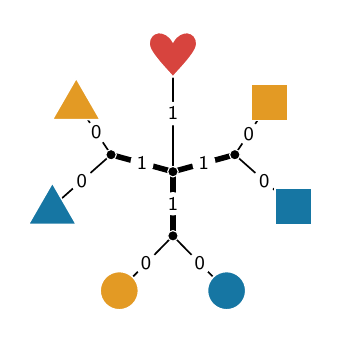
\begin{tikzpicture}[x=1.0cm,y=1.0cm,baseline=(current bounding box.center)]
\coordinate (v1) at (1.53153,-0.34956);
\coordinate (v2) at (-1.53153,-0.34956);
\coordinate (v3) at (0.68160,-1.41535);
\coordinate (v4) at (1.22819,0.97945);
\coordinate (v5) at (-1.22819,0.97945);
\coordinate (v6) at (-0.68160,-1.41535);
\coordinate (v7) at (0.00000,1.57092);
\coordinate (v8) at (0.78609,0.31154);
\coordinate (v9) at (-0.78609,0.31154);
\coordinate (v10) at (0.00000,-0.71909);
\coordinate (v11) at (0.00000,0.09601);
\draw[g2tree internal] (v8)--(v11);
\draw[g2tree internal] (v9)--(v11);
\draw[g2tree internal] (v10)--(v11);
\draw[g2tree pendant] (v1)--(v8);
\draw[g2tree pendant] (v2)--(v9);
\draw[g2tree pendant] (v3)--(v10);
\draw[g2tree pendant] (v4)--(v8);
\draw[g2tree pendant] (v5)--(v9);
\draw[g2tree pendant] (v6)--(v10);
\draw[g2tree pendant] (v7)--(v11);
\node[g2tree weight,font={\sffamily\fontsize{7.5}{8}\selectfont}] at (0.39304,0.20378) {1};
\node[g2tree weight,font={\sffamily\fontsize{7.5}{8}\selectfont}] at (-0.39304,0.20377) {1};
\node[g2tree weight,font={\sffamily\fontsize{7.5}{8}\selectfont}] at (0.00000,-0.31154) {1};
\node[g2tree weight,font={\sffamily\fontsize{7.5}{8}\selectfont}] at (1.15881,-0.01901) {0};
\node[g2tree weight,font={\sffamily\fontsize{7.5}{8}\selectfont}] at (-1.15881,-0.01901) {0};
\node[g2tree weight,font={\sffamily\fontsize{7.5}{8}\selectfont}] at (0.34080,-1.06722) {0};
\node[g2tree weight,font={\sffamily\fontsize{7.5}{8}\selectfont}] at (0.96293,0.57871) {0};
\node[g2tree weight,font={\sffamily\fontsize{7.5}{8}\selectfont}] at (-0.97227,0.59282) {0};
\node[g2tree weight,font={\sffamily\fontsize{7.5}{8}\selectfont}] at (-0.34080,-1.06722) {0};
\node[g2tree weight,font={\sffamily\fontsize{7.5}{8}\selectfont}] at (0.00000,0.83346) {1};
\node[g2tree vertex] at (v8) {};
\node[g2tree vertex] at (v9) {};
\node[g2tree vertex] at (v10) {};
\node[g2tree vertex] at (v11) {};
\node[g2tree dark,rectangle,minimum size=4.657500000000001mm,font={\sffamily\fontsize{9}{9}\selectfont\bfseries}] at (v1) {};
\begin{scope}[shift={(v2)},scale=1.0125000000000002,transform shape]
\path[fill=g2TaxonBlue,draw=white,line width=.55pt,line join=round] (0mm,3.0mm)--(-3.0mm,-2.2mm)--(3.0mm,-2.2mm)--cycle;
\end{scope}
\node[g2tree dark,circle,minimum size=4.86mm,font={\sffamily\fontsize{9}{9}\selectfont\bfseries}] at (v3) {};
\node[g2tree light,rectangle,minimum size=4.657500000000001mm,font={\sffamily\fontsize{9}{9}\selectfont\bfseries}] at (v4) {};
\begin{scope}[shift={(v5)},scale=1.0125000000000002,transform shape]
\path[fill=g2TaxonYellow,draw=white,line width=.55pt,line join=round] (0mm,3.0mm)--(-3.0mm,-2.2mm)--(3.0mm,-2.2mm)--cycle;
\end{scope}
\node[g2tree light,circle,minimum size=4.86mm,font={\sffamily\fontsize{9}{9}\selectfont\bfseries}] at (v6) {};
\begin{scope}[shift={(v7)},scale=1.0125000000000002,transform shape]
\path[fill=g2HeartRed,draw=white,line width=.55pt]
  (0mm,-2.7mm)..controls(-.45mm,-2.1mm)and(-3.0mm,.35mm)..(-3.0mm,1.45mm)
  ..controls(-3.0mm,3.2mm)and(-.9mm,3.4mm)..(0mm,1.75mm)
  ..controls(.9mm,3.4mm)and(3.0mm,3.2mm)..(3.0mm,1.45mm)
  ..controls(3.0mm,.35mm)and(.45mm,-2.1mm)..(0mm,-2.7mm)--cycle;
\end{scope}
\end{tikzpicture}
\endgroup
\par}
\end{minipage}}
 & 
\begin{minipage}[t][4.1325cm][t]{\linewidth}
\noindent\textcolor{g2TreeRule}{\rule{\linewidth}{1pt}}\par
\noindent\textcolor[HTML]{000000}{\smash[b]{\textpdfrender{TextRenderingMode=FillStroke,LineWidth=.5pt}{\Large\bfseries\boldmath \(\epsilon\)}{\large(3)}}}\par
\vskip -2.5mm
{\centering
\begingroup
\definecolor{g2TaxonBlue}{HTML}{1676A3}
\definecolor{g2TaxonYellow}{HTML}{E39A24}
\definecolor{g2HeartRed}{HTML}{D7443E}
\tikzset{
  g2tree pendant/.style={draw=black,line width=.6pt,line cap=round},
  g2tree internal/.style={draw=black,line width=2pt,line cap=round},
  g2tree vertex/.style={circle,fill=black,draw=white,line width=.4pt,inner sep=0pt,minimum size=3.8pt},
  g2tree dark/.style={fill=g2TaxonBlue,draw=white,line width=.55pt,text=white,inner sep=0pt},
  g2tree light/.style={fill=g2TaxonYellow,draw=white,line width=.55pt,text=white,inner sep=0pt},
  g2tree weight/.style={circle,fill=white,draw=none,text=black,inner sep=.15pt,minimum size=8.5pt},
  g2tree aligned pendant/.style={fill=white,text=black,inner sep=.7pt,sloped,above=1pt,font={\sffamily\fontsize{7.5}{8}\selectfont}},
  g2tree aligned internal/.style={fill=white,text=black,inner sep=1pt,sloped,above=1pt,font={\sffamily\fontsize{7.5}{8}\selectfont\bfseries}},
}
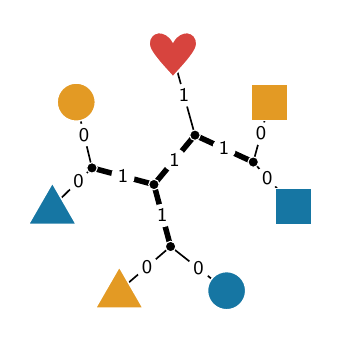
\begin{tikzpicture}[x=1.0cm,y=1.0cm,baseline=(current bounding box.center)]
\coordinate (v1) at (1.53153,-0.34956);
\coordinate (v2) at (-1.53153,-0.34956);
\coordinate (v3) at (0.68160,-1.41535);
\coordinate (v4) at (1.22819,0.97945);
\coordinate (v5) at (-0.68160,-1.41535);
\coordinate (v6) at (-1.22819,0.97945);
\coordinate (v7) at (0.00000,1.57092);
\coordinate (v8) at (1.01993,0.21810);
\coordinate (v9) at (-1.02847,0.14386);
\coordinate (v10) at (-0.03013,-0.85448);
\coordinate (v11) at (0.27985,0.55968);
\coordinate (v12) at (-0.24117,-0.06717);
\draw[g2tree internal] (v8)--(v11);
\draw[g2tree internal] (v9)--(v12);
\draw[g2tree internal] (v10)--(v12);
\draw[g2tree internal] (v11)--(v12);
\draw[g2tree pendant] (v1)--(v8);
\draw[g2tree pendant] (v2)--(v9);
\draw[g2tree pendant] (v3)--(v10);
\draw[g2tree pendant] (v4)--(v8);
\draw[g2tree pendant] (v5)--(v10);
\draw[g2tree pendant] (v6)--(v9);
\draw[g2tree pendant] (v7)--(v11);
\node[g2tree weight,font={\sffamily\fontsize{7.5}{8}\selectfont}] at (0.64989,0.38889) {1};
\node[g2tree weight,font={\sffamily\fontsize{7.5}{8}\selectfont}] at (-0.63482,0.03835) {1};
\node[g2tree weight,font={\sffamily\fontsize{7.5}{8}\selectfont}] at (-0.13565,-0.46082) {1};
\node[g2tree weight,font={\sffamily\fontsize{7.5}{8}\selectfont}] at (0.01934,0.24625) {1};
\node[g2tree weight,font={\sffamily\fontsize{7.5}{8}\selectfont}] at (1.19899,0.01942) {0};
\node[g2tree weight,font={\sffamily\fontsize{7.5}{8}\selectfont}] at (-1.20052,-0.02489) {0};
\node[g2tree weight,font={\sffamily\fontsize{7.5}{8}\selectfont}] at (0.32573,-1.13491) {0};
\node[g2tree weight,font={\sffamily\fontsize{7.5}{8}\selectfont}] at (1.11885,0.57974) {0};
\node[g2tree weight,font={\sffamily\fontsize{7.5}{8}\selectfont}] at (-0.33022,-1.11283) {0};
\node[g2tree weight,font={\sffamily\fontsize{7.5}{8}\selectfont}] at (-1.12833,0.56166) {0};
\node[g2tree weight,font={\sffamily\fontsize{7.5}{8}\selectfont}] at (0.13992,1.06530) {1};
\node[g2tree vertex] at (v8) {};
\node[g2tree vertex] at (v9) {};
\node[g2tree vertex] at (v10) {};
\node[g2tree vertex] at (v11) {};
\node[g2tree vertex] at (v12) {};
\node[g2tree dark,rectangle,minimum size=4.657500000000001mm,font={\sffamily\fontsize{9}{9}\selectfont\bfseries}] at (v1) {};
\begin{scope}[shift={(v2)},scale=1.0125000000000002,transform shape]
\path[fill=g2TaxonBlue,draw=white,line width=.55pt,line join=round] (0mm,3.0mm)--(-3.0mm,-2.2mm)--(3.0mm,-2.2mm)--cycle;
\end{scope}
\node[g2tree dark,circle,minimum size=4.86mm,font={\sffamily\fontsize{9}{9}\selectfont\bfseries}] at (v3) {};
\node[g2tree light,rectangle,minimum size=4.657500000000001mm,font={\sffamily\fontsize{9}{9}\selectfont\bfseries}] at (v4) {};
\begin{scope}[shift={(v5)},scale=1.0125000000000002,transform shape]
\path[fill=g2TaxonYellow,draw=white,line width=.55pt,line join=round] (0mm,3.0mm)--(-3.0mm,-2.2mm)--(3.0mm,-2.2mm)--cycle;
\end{scope}
\node[g2tree light,circle,minimum size=4.86mm,font={\sffamily\fontsize{9}{9}\selectfont\bfseries}] at (v6) {};
\begin{scope}[shift={(v7)},scale=1.0125000000000002,transform shape]
\path[fill=g2HeartRed,draw=white,line width=.55pt]
  (0mm,-2.7mm)..controls(-.45mm,-2.1mm)and(-3.0mm,.35mm)..(-3.0mm,1.45mm)
  ..controls(-3.0mm,3.2mm)and(-.9mm,3.4mm)..(0mm,1.75mm)
  ..controls(.9mm,3.4mm)and(3.0mm,3.2mm)..(3.0mm,1.45mm)
  ..controls(3.0mm,.35mm)and(.45mm,-2.1mm)..(0mm,-2.7mm)--cycle;
\end{scope}
\end{tikzpicture}
\endgroup
\par}
\vskip 0pt plus 1filll
\nointerlineskip\noindent\smash{\rlap{char\ 2}}\par
\end{minipage}
\\[0.19mm]
\end{tabular}
\endgroup
